
\section{Konzeption der Simulationsumgebung}\label{sec:SimEnv}
Nachdem die grundlegenden, konzeptionellen Entscheidungen für die Umsetzung des Simulators
getroffen sind, werden nun die Datenstrukturen und Algorithmen im Detail ausgearbeitet.
Die Umgebung simuliert ein steuerbares Fahrzeug, das statischen und dynamischen Hindernissen
ausweichen soll. Bei den Hindernissen handelt es sich jeweils um stationäre Gebäude
und Fußgänger, die sich in einer 2D Ebene bewegen.
Die Aktuatoren und Sensoren des Fahrzeugs werden in Form eines Markov Decision Process
bereitgestellt, um die Steuerung des Fahrzeugs durch einen Agent zu ermöglichen.
Im folgenden werden Aufbau und Funktionsweise der Simulationsumgebung beschrieben.

\subsection{Simulationsablauf}
Zu Beginn wählt die Simulationsumgebung aus einer Menge vorgegebener Routen
eine zufällige Route aus und positioniert das Fahrzeug in der Startzone der Route.
Anschließend steuert der Agent das Fahrzeug von Wegpunkt zu Wegpunkt, bis es am Routenziel ist.
Um das Auswendiglernen der Route zu vermeiden, werden Start- und Zielpositionen zufällig
variiert. Ein Wegpunkt gilt als erreicht, wenn sich das Fahrzeug zu einem diskreten
Simulationszeitpunkt nah genug am Wegpunkt befindet. Kollidiert das Fahrzeug hingegen
mit einem Fußgänger oder einem Hindernis, wird die Navigation der aktuellen Route
abgebrochen. In diesem Fall oder beim Erreichen des Routenziels startet die Navigation
einer neuen Route.\\

Die Simulation setzt sich aus einer Abfolge vieler, kleiner Simulationsschritte
zusammen, die jeweils den Systemzustand zu einem diskreten Zeitpunkt $t$ repräsentieren.
Zwischen zwei aufeinanderfolgenden Zeitschritten vergeht Zeit in Höhe des Zeitintervalls
$\Delta t$, das je nach Anzahl der vom Fahrzeug durchführbaren Aktionen, der sog.
Aktionsfrequenz, konfiguriert werden kann.
Pro Zeitschritt wird zunächst von außen eine Aktion für das Fahrzeug gewählt, mit der
das Fahrzeug entsprechend seiner Kinematik fährt. Daraufhin bewegen sich alle Fußgänger
gemäß der Kräfte des Social Force Modells. Abschließend wird der neue Systemzustand
bestimmt, mithilfe der Fahrzeugsensorik aus Sicht des Fahrzeugs erfasst und nach außen
propagiert, damit die nächste Aktion gewählt werden kann.

\subsection{Aktuatoren und Action Spaces}
Die Aktuatoren modellieren die Kontrolle bezüglich der lateralen und longitudinalen
Bewedungsdynamik des Fahrzeugs zum Beschleunigen, Bremsen und Lenken. Diese sind
spezifisch für die zugehörige Fahrzeugkinematik.\\

Im Fall des Differentialgetriebenen Fahrens werden die Aktuatoren als lineare
Geschwindigkeit $v$ und Winkelgeschwindigkeit $\omega$ definiert \ref{sec:DiffDrive}.
Folglich ergibt sich ein Action Space von $[0, v_{max}]$ für die lineare
Geschwindigkeit und ein Action Space von $[-\omega_{max}, \omega_{max}]$
für die Winkelgeschwindigkeit des Fahrzeugs. Da sich das Fahrzeug auf der
Stelle drehen kann, ist kein Rückwärtsfahren vorgesehen.\\

Beim Fahrradmodell werden die Aktuatoren als Beschleunigung $a$ und Lenkwinkel
$\delta$ modelliert. \ref{sec:Bicycle} Somit ergibt sich ein Action Space von
$[-a_{max}, a_{max}]$ für die Beschleunigung und ein Action Space von
$[-\delta_{max}, \delta_{max}]$ für den Lenkwinkel des Fahrzeugs. Aufgrund der
negativen Beschleunigung kann rückwärts gefahren werden, was jedoch deaktivierbar ist.

\subsection{Sensoren und Observation Spaces}
Als Sensoren kommen ein radialer Strahlensensor (LiDAR), ein Positionssensor (GPS)
und ein Sensor für die Bewegungsdynamik des Fahrzeugs zum Einsatz.\\

Eine Observation setzt sich aus mehreren Komponenten zusammen. Sie besteht
zum einen aus der Bewegungsdynamik des Fahrzeugs, zum anderen aus
der relativen Position des Fahrzeugs zum angepeilten Zielpunkt als Polarvektor.
Zusätzlich gehen die Entfernungen des Strahlensensors in die Observation ein.
Somit ergeben sich für die Bewegungsdynamik des Fahrzeugs Observation Spaces
$[0, v_{max}]$ für die Geschwindigkeit und $[-\omega_{max}, \omega_{max}]$
bzw. $[-\phi_{max}, \phi_{max}]$ für die Lenkung ähnlich zu den Aktuatoren.

\begin{figure}[h]
  \centering
  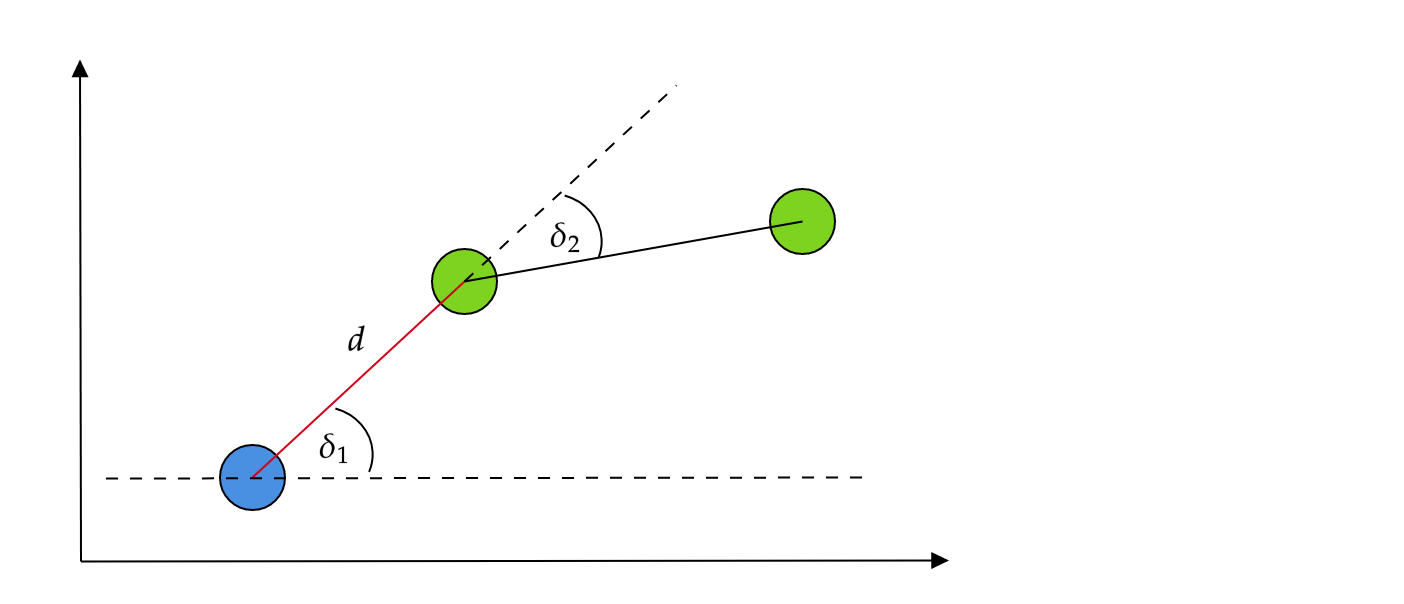
\includegraphics[width = 1.0\textwidth]{imgs/goal_sensor}
  \caption{Sensorik der Zielpeilung zwischen dem Fahrzeug (blau) und den nächsten beiden
  Wegpunkten (grün).   Dem Agent steht das Tupel $(d, \delta_1, \delta_2)$ bezüglich Zieldistanz,
  Trajektorie und Orientierung im Koordinatensystem zur Verfügung.}
  \label{fig:goal_sensor}
\end{figure}

Die Observation Spaces der Zielpeilung sind $[0, d_{max}]$, $[-\pi, \pi]$, wobei die maximal
mögliche Zielentfernung $d_{max} = \sqrt{(h_{map})^2 + (w_{map})^2}$ anhand der Ausmaße der
Karte bzgl. deren Breite $w_{map}$ und Höhe $h_{map}$ beschrieben wird. Der LiDAR-Sensor sendet
seine Strahlen gleichmäßig verteilt über den Öffnungswinkel $\varphi$ aus. Jeder Strahl wird
durch einen Observation Space von $[0, s_{max}]$ mit fester, maximaler Scanreichweite $s_{max}$
repräsentiert. Um die Route zielgerichteter fahren zu können, wird die Peilung des übernächsten
Ziels als Winkel zwischen der Fahrzeugposition und dem nächsten und übernächsten Zielpunkt
bereitgestellt, wie in Abbildung \ref{fig:goal_sensor} zu sehen ist. Dies entspricht
ebenfalls einem Observation Space von $[-\pi, \pi]$.\\

\begin{figure}[h]
  \centering
  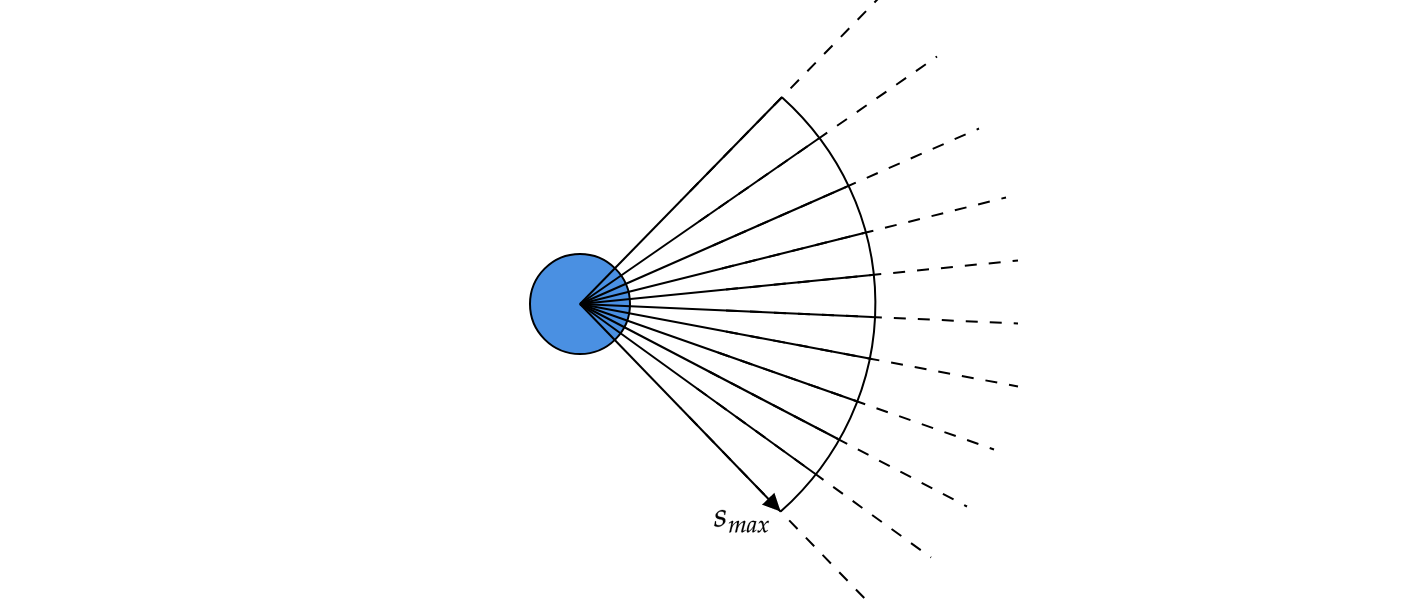
\includegraphics[width = 0.65\textwidth]{imgs/lidar_sensor}
  \caption{Schaubild eines LiDAR-Sensors mit Öffnungswinkel $\varphi$  und maximaler Scandistanz $s_{max}$.}
  \label{fig:linseg_circle_intersect}
\end{figure}

Da es unmöglich ist, die Bewegungsdynamiken der Fußgänger aus einem Standbild
erfasster Entfernungen durch den Strahlensensor abzuleiten, stehen dem Fahrzeug
immer mindestens die Strahlendaten der letzten 3 Zeitschritte zur Verfügung.

\subsection{Kartenmaterial: Statische und dynamische Entitäten}
Das Kartenmaterial setzt sich aus Vektorgrafiken zusammen, die die Fußgänger,
Hindernisse und das Fahrzeug repräsentieren. Hierbei werden Fußgänger und das
Fahrzeug als Kreise und Hindernisse als Liniensegmente in der 2D Ebene modelliert,
was der Umsetzung von PySocialForce entspricht.\\

Hindernisse haben eine statische Position und können verwendet werden,
um zusammengesetzte Entitäten wie Polygone oder aneinandergefügte Liniensegmente
zu repräsentieren. Fußgänger und Fahrzeuge sind hingegen dynamische Entitäten
und können sich auf der Karte bewegen.

\subsection{Kollisionserkennung}
Bei der Kollisionserkennung wird geprüft, ob das Fahrzeug mit anderen Entitäten
wie beispielsweise Fußgängern oder Hindernissen zusammengestoßen ist.
Dies entspricht einem Überlappen der geometrischen Formen, die die jeweiligen
Entitäten repräsentieren. Im Folgenden werden die dafür benötigten Formeln
hergeleitet und bezüglich effizienter Berechenbarkeit optimiert.

\subsubsection{Kollisionen zwischen Fahrzeug und Fußgängern}
Kollisionen zwischen dem Fahrzeug und Fußgängern können sehr einfach erkannt werden.
Als Distanzmetrik dient hierbei die euklidische Distanz zwischen den Kreiszentren
$C_{ped} = (x_{ped}, y_{ped})^T$ und $C_{veh} = (x_{veh}, y_{veh})^T$.
Ist die Distanz kleiner als die Summe der Kreisradien, schneiden sich die Kreise
und es liegt eine Kollision vor, wie in Abbildung \ref{fig:circle_intersect}
zu sehen ist. Die Konstellation in Fall 1, bei der sich ein Kreis vollständig innerhalb
des anderen Kreises befindet, wird ebenfalls als eine Kollision betrachtet.\\

\begin{figure}[h]
  \centering
  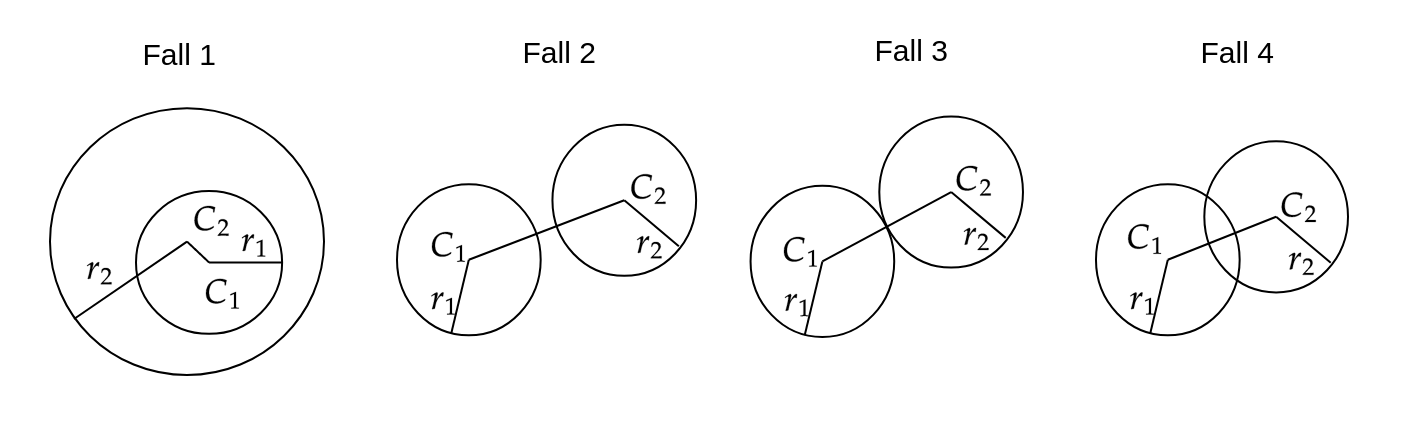
\includegraphics[width = 1.0\textwidth]{imgs/circle_intersections}
  \caption{Fallbetrachtung möglicher Schnittpunkte zwischen zwei Kreisen mit Zentren $C_1$, $C_2$
  und Radien $r_1$, $r_2$. Nur in Fall 2 liegt keine Kollision vor.}
  \label{fig:circle_intersect}
\end{figure}

\begin{equation}
\begin{aligned}
dist(C_{ped}, C_{veh}) \le r_{ped} + r_{veh}
\end{aligned}
\end{equation}

\begin{equation}
\begin{aligned}
dist(C_{ped}, C_{veh}) = \lVert C_{veh} - C_{ped} \rVert
= \sqrt{(x_{ped} - x_{veh})^2 + (y_{ped} - y_{veh})^2}
\end{aligned}
\end{equation}

Um die kostspielige Quadratwurzelberechnung zu sparen, wird die Formel
auf beiden Seiten der Ungleichung quadriert. Die zusätzlich hinzugefügte Lösung
im negativen Wertebereich stellt kein Problem dar, da Distanzen und Kreisradien
immer $\ge 0$ sind. Somit ergibt sich:

\begin{equation}
\begin{aligned}
dist(C_{ped}, C_{veh})^2 \le (r_{ped} + r_{veh})^2
\end{aligned}
\end{equation}

\begin{equation}
\begin{aligned}
(x_{ped} - x_{veh})^2 + (y_{ped} - y_{veh})^2 \le (r_{ped} + r_{veh})^2
\end{aligned}
\end{equation}

Pro Zeitschritt muss für jeden der n Fußgänger geprüft werden, ob er mit dem Fahrzeug
kollidiert, was in linearer Zeit $O(n)$ mit $O(1)$ zusätzlichem Speicher durchgeführt
werden kann. Die damit verbundenen Operationen können zudem sehr effizient und
unabhänging voneinander berechnet werden.

\subsubsection{Kollisionen zwischen Fahrzeug und statischen Hindernissen}
Auch Kollisionen des Fahrzeugs mit Hindernissen müssen berechnet werden. Hierfür wird
die Menge aller auf dem Kreisbogen befindlichen Punkte mit der Menge aller auf
dem Liniensegment (Hindernis) befindlichen Punkten geschnitten, um alle potentiellen
Schnittpunkte zu bestimmen.\\

\begin{figure}[h]
  \centering
  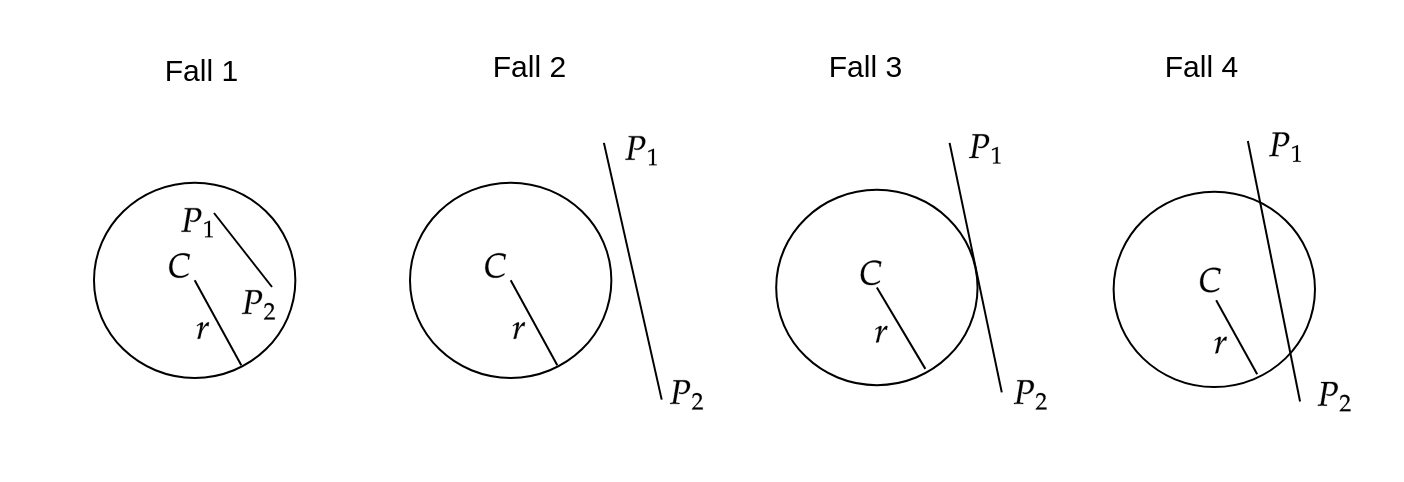
\includegraphics[width = 1.0\textwidth]{imgs/line_circle_intersections}
  \caption{Fallbetrachtung möglicher Schnittpunkte zwischen einem Liniensegment
  zwischen $P_1$, $P_2$ und einem Kreis mit Zentrum $C$ und Radius $r$.
  Nur in Fall 2 keine Kollision vor.}
  \label{fig:linseg_circle_intersect}
\end{figure}

Anhand der Kreisgleichung befindet sich ein Punkt $P$ genau dann auf der Kreislinie,
wenn die Distanz zwischen der Kreismitte $C$ und $P$ dem Radius $r$ des Kreises
entspricht. Vereinfachend wird die Kreismitte zum Ursprung verschoben, sodass
der Abstand zwischen Kreismitte und $P$ genau $\lVert P \rVert$ beträgt.

\begin{equation}
\begin{aligned}
M_{circle} = \{ P \epsilon R^2 | r = \lVert P \rVert \}
\end{aligned}
\end{equation}

Ein Hindernis ist als Liniensegment zwischen zwei Endpunkten $(P_1, P_2)$ definiert.
Die zugehörige Geradengleichung ergibt sich durch einen Punkt auf der Gerade plus
ein Vielfaches $\mu$ eines Richtungsvektors. In diesem Fall ist die Gerade durch
$P_1 - C$ und den Richtungsvektor $P_2 - P_1$ gegeben. Um ausschließlich auf
der Gerade befindliche Punkte innerhalb des Liniensegments zu erhalten, wird das
Vielfache $\mu$ des Richtungsvektors auf $0 \le \mu \le 1$ beschränkt.

\begin{equation}
\begin{aligned}
M_{line} = \{ \mu (P_2 - P_1) + (P_1 - C) | \mu \epsilon R \land 0 \le \mu \le 1 \}
\end{aligned}
\end{equation}

Nun kann die Schnittmenge der beiden Punktmengen $M_{line} \cap M_{circle}$
bestimmt werden, um auf Schnittpunkte bzw. Kollisionen zu prüfen. Hierfür wird
der von $P_1$ nach $P_2$ zeigende Vektor als $s = P_2 - P_1$ und der von
$C$ nach $P_1$ zeigende Vektor als $t = P_1 - C$ notiert.

\begin{equation}
\begin{aligned}
r = {\lVert \mu s + t \rVert} &\iff r^2 = {\lVert \mu s + t \rVert}^2\\
&\iff r^2 = (\mu s + t) \cdot (\mu s + t)\\
&\iff r^2 = \mu^2 s \cdot s + 2 \mu s \cdot t + t \cdot t\\
&\iff 0 = \mu^2 s \cdot s + 2 \mu s \cdot t + t \cdot t - r^2
\end{aligned}
\end{equation}

\begin{equation}
\begin{aligned}
a = s \cdot s, b = 2 s \cdot t, c = t \cdot t - r^2
\end{aligned}
\end{equation}

Dieses von $\mu$ abhängige Gleichungssystem führt zu einer quadratischen Gleichung
mit 0 bis 2 Lösungen, die durch die Lösungsformel für quadratische Gleichungen
bestimmt werden können.

\begin{equation}
\begin{aligned}
\mu_{1,2} = \frac{-b \pm \sqrt{D}}{2 a}, D = b^2 - 4 a c
\end{aligned}
\end{equation}

Das Gleichungssystem hat in den reellen Zahlen 0 Lösungen, wenn $D < 0$,
1 Lösung, wenn $D = 0$ und 2 Lösungen, wenn $D > 0$. Wie in Abbildung
\ref{fig:linseg_circle_intersect} dargestellt, liegt eine Kollision vor,
sofern $0 \le \mu \le 1$. Zudem besteht ein Sonderfall
einer Kollision, wenn sich das Liniensegment vollständig innerhalb des Kreises
befindet, was gesondert geprüft werden muss. Da jede Prüfung in konstanter Zeit
möglich ist, ergibt sich für $o$ Hindernisse eine Zeitkomplexität von $0(o)$;
die Speicherkomplexität ist konstant.

\subsection{Simulation radialer Strahlensensoren (LiDAR)}
Ein radialer Strahlensensor sendet eine gewisse Anzahl an Strahlen aus, deren
Ausrichtungen gleichmäßig über den Öffnungsbereich des Sensors verteilt sind.
Für jeden Strahl muss die Distanz zwischen der Strahlenquelle und der
nächstgelegenen, getroffenen Entität innerhalb des Suchradius berechnet werden.
Es ergibt sich demnach für $r$ Strahlen, $p$ Fußgänger und $o$ Hindernisse eine
Zeitkomplexität von $O({r (p + o)})$ und eine Speicherkomplexität von $O(r)$.

\subsubsection{Entfernungen zu Fußgängern}
Um die Entfernung zwischen einer Strahlenquelle und einem vom Strahl getroffenen
Fußgänger zu berechnen, wird der Fußgänger als Kreis und der Strahl als eine von
der Strahlenquelle ausgehende Halbgerade modelliert. Die Richtung des Strahls
ist durch den Einheitsvektor $v_{ray}$ gegeben.\\

Die Formel zur Kollisionsberechnung zwischen einer Linie und einem Kreis wurde
bereits für Kollisionen zwischen Fahrzeugen und Hindernissen hergeleitet. Im Gegensatz
zum vorherigen Anwendungsfall ist aber nicht nur relevant, ob eine Kollision vorliegt,
sondern auch wie weit sie entfernt ist.
Hierfür werden ebenfalls $\mu_{1,2}$ bestimmt und anschließend in die Formel $P_{Gerade}$
eingesetzt, um die beiden Schnittpunkte $S_1, S_2$ zu bestimmen. Falls es
keine Schnittpunkte gibt, ist die Entfernung $\infty$. Bei exakt einem Schnittpunkt
ist $S_1 = S_2$, was o.B.d.A. nicht weiter betrachtet werden muss.\\

Nun kann die kürzeste Entfernung von der Strahlenquelle zu den Schnittpunkten
$S_1, S_2$ als  $min(dist(P_{sensor}, S_1), dist(P_{sensor}, S_2))$ bestimmt werden.
Allerdings ist hierbei zu beachten, dass der Vektor von der Strahlenquelle zum
Schnittpunkt ein positives Vielfaches des Strahlenvektors $v_{ray}$ sein muss,
da sich der Strahl nur in diese Richtung ausbreitet. Dies kann durch $\mu \ge 0$
geprüft werden.

\begin{equation}
\begin{aligned}
\mu_{1,2} = \frac{-b \pm \sqrt{D}}{2 a}, D = b^2 - 4 a c\\
a = s \cdot s, b = 2 s \cdot t, c = t \cdot t - r^2
\end{aligned}
\end{equation}

Um sich im Fall, dass keine Kollision vorliegt, die Quadratwurzelberechnung
$\sqrt{D}$ zu sparen, wird nochmals die Lösungsformel für quadratische Gleichungen
betrachtet. Da $a = \lVert s \rVert^2 \implies 2a > 0$, gibt es genau dann keine Kollision,
wenn entweder $D < 0$ oder $-b \pm \sqrt{D} < 0$.

\begin{equation}
\begin{aligned}
-b \pm \sqrt{D} < 0 \iff -b + \sqrt{D} < 0 \iff \sqrt{D} < b \iff b > 0 \land b^2 > D
\end{aligned}
\end{equation}

Somit kann die Prüfung auf $\mu < 0$ durch $b > 0$ und $b^2 > D$ ersetzt werden.

\subsubsection{Entfernungen zu Hindernissen}
Zur Entfernungsberechnung zwischen einer Strahlenquelle und Hindernissen wird
eine neue Berechnungsformel benötigt, die eine Halbgerade (Strahl) mit einen
Liniensegment (Hindernis) schneidet.
Die Halbgerade ist gegeben durch die Position der Strahlenquelle $P_{sensor}$ und
den Richtungsvektor $v_{ray}$ des Strahls als Einheitsvektor; das Liniensegment zwischen
$P_1$ und $P_2$ ist durch den Punkt $P_1$ und den Richtungsvektor $v_{seg} = P_2 - P_1$
definiert. Bei der Halbgerade sind nur Vielfache $\tau \ge 0$ des Richtungsvektors
erlaubt, beim Liniensegment nur Vielfache $\mu \in [0, 1]$.\\

\begin{figure}[h]
  \centering
  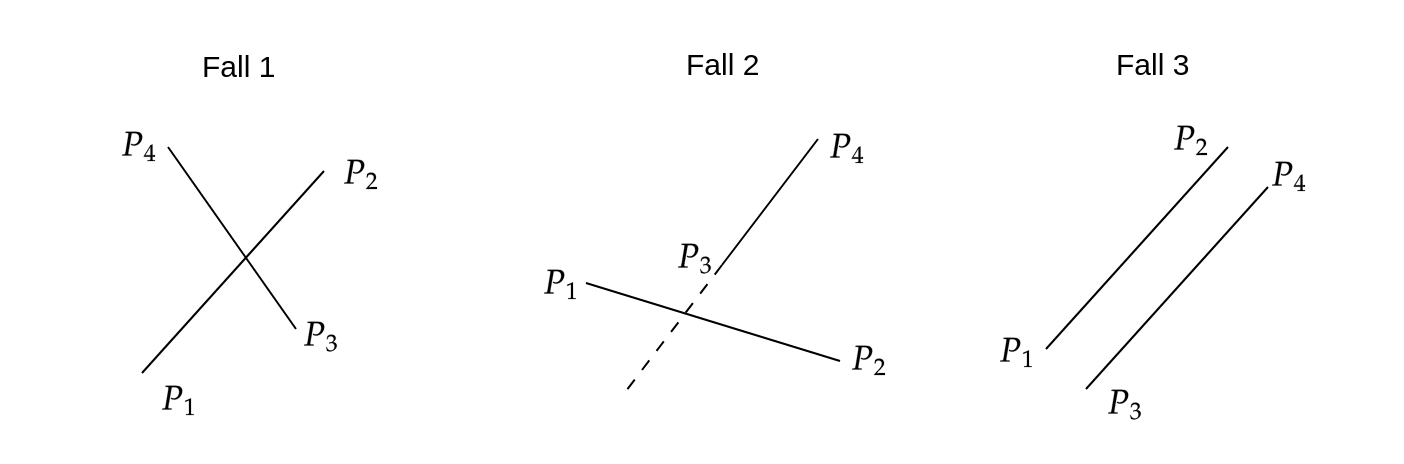
\includegraphics[width = 1.0\textwidth]{imgs/lineseg_intersections}
  \caption{Fallbetrachtung möglicher Schnittpunkte zwischen zwei Liniensegmenten,
  jeweils definiert durch ihre Endpunkte $P_1$, $P_2$ bzw. $P_3$, $P_4$.
  Parallele Linien wie in Fall 3 schneiden sich nicht. Außerdem sind die
  Enden der Segmente zu beachten.}
  \label{fig:linseg_intersect}
\end{figure}

Nun können die beiden Punktmengen $M_{ray}$ und $M_{obstacle}$ aufgestellt und deren
Schnittmenge $M_{ray} \cap M_{obstacle}$ bestimmt werden, um alle Schnittpunkte zu erhalten.

\begin{equation}
\begin{aligned}
M_{ray} = \{ P_{sensor} + \tau v_{ray} | \tau \in R, \tau > 0 \}
\end{aligned}
\end{equation}

\begin{equation}
\begin{aligned}
M_{obstacle} = \{ P_1 + \mu v_{seg} | \mu \in R, 0 \le \mu \le 1 \}
\end{aligned}
\end{equation}

\begin{equation}
\begin{aligned}
M_{ray} \cap M_{obstacle} =
\{ P_1 + \mu v_{seg} | \mu \in R, P_{sensor} + \tau v_{ray} = P_1 + \mu v_{seg} \}
\end{aligned}
\end{equation}

Dies ergibt ein von den Unbekannten $\tau$ und $\mu$ abhängiges Gleichungssystem,
bestehend aus zwei Gleichungen bezüglich der linear unabhängigen x/y Koordinaten
der Vektoren. Das Gleichungssystem ist also eindeutig lösbar.

\begin{equation}
\begin{aligned}
&P_{sensor} = (x_{sensor}, y_{sensor})^T, P_1 = (x_1, y_1)^T,\\
&v_{ray} = (x_{ray}, y_{ray})^T, v_{seg} = (x_{seg}, y_{seg})^T\\
&v_{diff} = (x_{diff}, y_{diff})^T = P_1 - P_{sensor}
\end{aligned}
\end{equation}

\begin{equation}
\begin{aligned}
I)& \, x_{sensor} + \tau x_{ray} = x_1 + \mu x_{seg}\\
II)& \, y_{sensor} + \tau y_{ray} = y_1 + \mu y_{seg}
\end{aligned}
\end{equation}

Durch Umformen ergeben sich folgende nach $\tau$ aufgelöste Gleichungen:

\begin{equation}
\begin{aligned}
I')& \, \tau = \frac{\mu x_{seg} + x_{diff}}{x_{ray}}\\
II')& \, \tau = \frac{\mu y_{seg} + y_{diff}}{y_{ray}}
\end{aligned}
\end{equation}

Nun wird $\tau$ durch Gleichsetzen eliminiert. Anschließend wird nach $\mu$ aufgelöst,
um die Lösung des Gleichungssystems zu bestimmen.

\begin{equation}
\begin{aligned}
\frac{\mu x_{seg} + x_{diff}}{x_{ray}} = \frac{\mu y_{seg} + y_{diff}}{y_{ray}}
\end{aligned}
\end{equation}

\begin{equation}
\begin{aligned}
\mu \frac{x_{seg}}{x_{ray}} + \frac{x_{diff}}{x_{ray}}
= \mu \frac{y_{seg}}{y_{ray}} + \frac{y_{diff}}{y_{ray}}
\end{aligned}
\end{equation}

\begin{equation}
\begin{aligned}
\mu \frac{x_{seg}}{x_{ray}} - \mu \frac{y_{seg}}{y_{ray}}
= \frac{y_{diff}}{y_{ray}} - \frac{x_{diff}}{x_{ray}}
\end{aligned}
\end{equation}

\begin{equation}
\begin{aligned}
\mu \left(\frac{x_{seg} y_{ray}}{x_{ray} y_{ray}} - \frac{x_{ray} y_{seg}}{x_{ray} y_{ray}}\right)
= \frac{x_{ray} y_{diff}}{x_{ray} y_{ray}} - \frac{y_{ray} x_{diff}}{x_{ray} y_{ray}}
\end{aligned}
\end{equation}

\begin{equation}
\begin{aligned}
\mu \frac{x_{seg} y_{ray} - x_{ray} y_{seg}}{x_{ray} y_{ray}}
= \frac{x_{ray} y_{diff} - y_{ray} x_{diff}}{x_{ray} y_{ray}}
\end{aligned}
\end{equation}

\begin{equation}
\begin{aligned}
\mu (x_{seg} y_{ray} - x_{ray} y_{seg}) = x_{ray} y_{diff} - y_{ray} x_{diff}
\end{aligned}
\end{equation}

\begin{equation}
\begin{aligned}
\mu = \frac{x_{ray} y_{diff} - y_{ray} x_{diff}}{x_{seg} y_{ray} - x_{ray} y_{seg}},
x_{seg} y_{ray} - x_{ray} y_{seg} \neq 0
\end{aligned}
\end{equation}

Wenn $x_{seg} y_{ray} - x_{ray} y_{seg} \neq 0$, ergibt sich der Schittpunkt
$S = P_1 + \mu v_{seg}$ durch Einsetzen von $\mu$ in $M_{obstacle}$.
$\tau$ kann über $\tau = \frac{\mu x_{seg} + x_{diff}}{x_{ray}}$ oder
$\tau = \frac{\mu y_{seg} + y_{diff}}{y_{ray}}$ bestimmt werden.
Nun muss noch überprüft werden, ob $0 \le \mu \le 1$ und $\tau \ge 0$. Ist dies der Fall,
trifft der Strahl das Hindernis nach einer Entfernung von $dist(P_{sensor}, S)$,
andernfalls ist die Distanz $\infty$.
Wenn $x_{seg} y_{ray} - x_{ray} y_{seg} = 0$, steht der Strahl parallel zum Hindernis
und verfehlt, da Hindernisse keine Tiefe besitzen.

\subsubsection{Nachbereitung der berechneten Entfernungen}
Nachdem die Kollisionsberechnungen für alle Strahlen und Entitäten durchgeführt wurden,
kann die minimale Entfernung $d_{ray}$ pro Strahl bestimmt werden.
Entfernungen, die noch auf $\infty$ initialisiert sind, da keine Kollision vorliegt,
werden mit $d_{ray} = min(d_{ray}, s_{max})$ auf die maximale Scanreichweite
des Sensors beschränkt.\\

Nun wird zur bisher perfekten Messung ein leichtes Rauschen hinzugefügt, was vor allem
für das Training einer Künstlichen Intelligenz wichtig ist, um Overfitting vorzubeugen.
Hierbei gehen Strahlen mit einer gewissen Wahrscheinlichkeit $P_{lost}$ ganz verloren,
sodass die gemessene Distanz der maximalen Scanreichweite entspricht.
Zudem können auch Messungen mit der Wahrscheinlichkeit $P_{corrupt}$ verfälscht werden,
sodass die Entfernung zufällig um einen gleichverteilten Faktor $f \in [0, 1]$
skaliert wird. Empfohlene Wahrscheinlichkeiten sind $P_{lost} = 0.005$
und $P_{corrupt} = 0.002$.

\subsection{Steuerung der Fußgänger}
Bezüglich der Simulation von realistischem Fußgängerverhalten, wird das Social Force Modell
aus Abschnitt \ref{sec:SocialForce} verwendet, um Fußgänger einzeln oder in Gruppen zu einem
Zielort zu bewegen.
Eine Gruppe ist am Ziel, wenn sich ihr Massenschwerpunkt $\frac{1}{n} \sum_{i=1}^n p_i$
zu einem diskreten Zeitpunkt $t$ nah genug am Zielpunkt befindet. O.B.d.A. sind einzelne
Fußgänger als eine Gruppe mit nur einem Fußgänger definiert. Da Fußgängerzonen und Gehwege
simuliert werden sollen, wird im Folgenden betrachtet, wie ein entsprechendes Verhalten
erzielbar ist.\\

Zur Simulation von Fußgängerzonen werden zunächst Zonen definiert, in denen sich
die Fußgänger aufhalten. Um ein Verhalten zu erzielen, bei dem die Fußgänger
durcheinander laufen, werden gleichverteilt zufällige Zielpunkte innerhalb
der Zone gewählt, zu denen die Fußgänger laufen. Sobald ein Ziel erreicht ist,
wird ein neues, zufälliges Ziel bestimmt.
Das stationäre Verhalten in Fußgängerzonen wird durch das zielgerichtete Laufen
von Routen ergänzt, was eher dem Fußgängerverhalten auf Gehwegen entspricht.
Ähnlich wie bei der Globalen Navigation des Fahrzeugs werden die Routen zwischen Start-
und Zielzone anhand von groben Wegpunkten vorgegeben. Sobald ein Wegpunkt erreicht ist,
wird der nächste angesteuert. Sind die Fußgänger am finalen Ziel innerhalb der
Zielzone, erscheinen sie wieder in der Startzone, um die Route erneut zu laufen.\\

Entsprechend der vorgegebenen Fußgängerdichte, d.h. Fußgänger pro Fläche, werden allen Routen
und Fußgängerzonen eine Anzahl an Fußgängern gemäß ihrer Fläche zugewiesen. Die Gehwegfläche
wird durch die Multiplikation der jeweiligen Routenlänge mit einer angenommenen Gehwegbreite
von 3-4 Metern geschätzt. Wie in Moussaïd et. al \cite{moussaid2010groupssf} beschrieben ist
die Größe der Gruppen poissonverteilt. Daher wird vor der Zuteilung der Fußgänger zunächst
die Anzahl der Gruppenmitglieder gemäß der Wahrscheinlichkeitsverteilung gezogen.
Anschließend werden die Massenschwerpunkte der Gruppen gleichverteilt innerhalb der
Fußgängerzonen bzw. entlang der Routen bestimmt und deren Gruppenmitglieder normalverteilt
um den Schwerpunkt positioniert.
